% The contents of this file is 
% Copyright (c) 2009-  Charles R. Severance, All Righs Reserved
% 한국어 번역 : 이광춘, 한정수

\chapter{네트워크 프로그램}
지금까지 책의 많은 예제는 파일을 읽고 파일의 정보를 찾는데 집중했지만, 
다양한 많은 정보의 원천이 인터넷에 있다.

이번 장에서는 웹브라우져로 가장하고 HTTP 프로토콜(HyperText Transport Protocol,HTTP)을 사용하여 웹페이지를 검색할 것이다. 
웹페이지 데이터를 읽고 파싱할 것이다.

\section{하이퍼 텍스트 전송 프로토콜(HyperText Transport Protocol - HTTP)}
웹에 동력을 공급하는 네트워크 프로토콜은 실제로 매우 단순하다.
파이썬에는 {\tt 소켓 (sockets)}이라고 불리는 내장 지원 모듈이 있다. 
파이썬 프로그램에서 소켓 모듈을 통해서 네트워크 연결을 하고, 데이터 검색을 매우 용이하게 한다.

{\bf 소켓(socket)}은 단일 소켓으로 두 프로그램 사이에 양방향 연결을 제공한다는 점을 제외하고 파일과 매우 유사하다.
동일한 소켓에 읽거나 쓸 수 있다. 
소켓에 무언가를 쓰게 되면, 소켓의 다른 끝에 있는 응용프로그램에 전송된다. 
소켓으로부터 읽게 되면, 다른 응용 프로그램이 전송한 데이터를 받게 된다.

하지만, 소켓의 다른쪽 끝에 프로그램이 어떠한 데이터도 전송하지 않았는데 소켓을 읽으려고 하면, 단지 앉아서 기다리기만 한다.
만약 어떠한 것도 보내지 않고 양쪽 소켓 끝의 프로그램 모두 기다리기만 한다면, 모두 매우 오랜 시간동안 기다리게 될 것이다.

인터넷으로 통신하는 프로그램의 중요한 부분은 특정 종류의 프로토콜을 공유하는 것이다.
프로토콜(protocol)은 정교한 규칙의 집합으로 누가 메시지를 먼저 보내고, 메세지로 무엇을 하며, 메시지에 대한 응답은 무엇이고, 다음에 누가 메세지를 보내고 등등을 포함한다.
이런 관점에서 소켓 끝의 두 응용프로그램이 함께 춤을 추고 있으니, 다른 사람 발을 밟지 않도록 확인해야 한다.

네트워크 프로토콜을 기술하는 문서가 많이 있다. 
하이퍼텍스트 전송 프로토콜(HyperText Transport Protocol)은 다음 문서에 기술되어 있다.

\url{http://www.w3.org/Protocols/rfc2616/rfc2616.txt}

매우 상세한 176 페이지나 되는 장문의 복잡한 문서다. 
흥미롭다면 시간을 가지고 읽어보기 바란다. 
RFC2616에 36 페이지를 읽어보면, GET 요청(request)에 대한 구문을 발견하게 된다. 
꼼꼼히 읽게 되면, 웹서버에 문서를 요청하기 하기 위해서, 80 포트로 {\tt www.py4inf.com} 서버에 
연결을 하고 나서 다음 양식 한 라인을 전송한다.

{\tt GET http://www.py4inf.com/code/romeo.txt HTTP/1.0 }

두번째 매개변수는 요청하는 웹페이지가 된다. 
그리고 또한 빈 라인도 전송한다. 
웹서버는 문서에 대한 헤더 정보와 빈 라인 그리고 문서 본문으로 응답한다.


\section{세상에서 가장 간단한 웹 브라우져(Web Browser)}
아마도 HTTP 프로토콜이 어떻게 작동하는지 알아보는 가장 간단한 방법은 매우 간단한 파이썬 프로그램을 작성하는 것이다.
웹서버에 접속하고 HTTP 프로토콜 규칙에 따라 문서를 요청하고 서버가 다시 보내주는 결과를 보여주는 것이다.

\beforeverb
\begin{verbatim}
import socket

mysock = socket.socket(socket.AF_INET, socket.SOCK_STREAM)
mysock.connect(('www.py4inf.com', 80))
mysock.send('GET http://www.py4inf.com/code/romeo.txt HTTP/1.0\n\n')

while True:
    data = mysock.recv(512)
    if ( len(data) < 1 ) :
        break
    print data

mysock.close()
\end{verbatim}
\afterverb
%

처음에 프로그램은 \url{www.py4inf.com} 서버에 80 포트로 연결한다.
''웹 브라우져'' 역할로 작성된 프로그램이 하기 때문에 HTTP 프로토콜은 GET 명령어를 공백 라인과 함께 보낸다.

\beforefig
\centerline{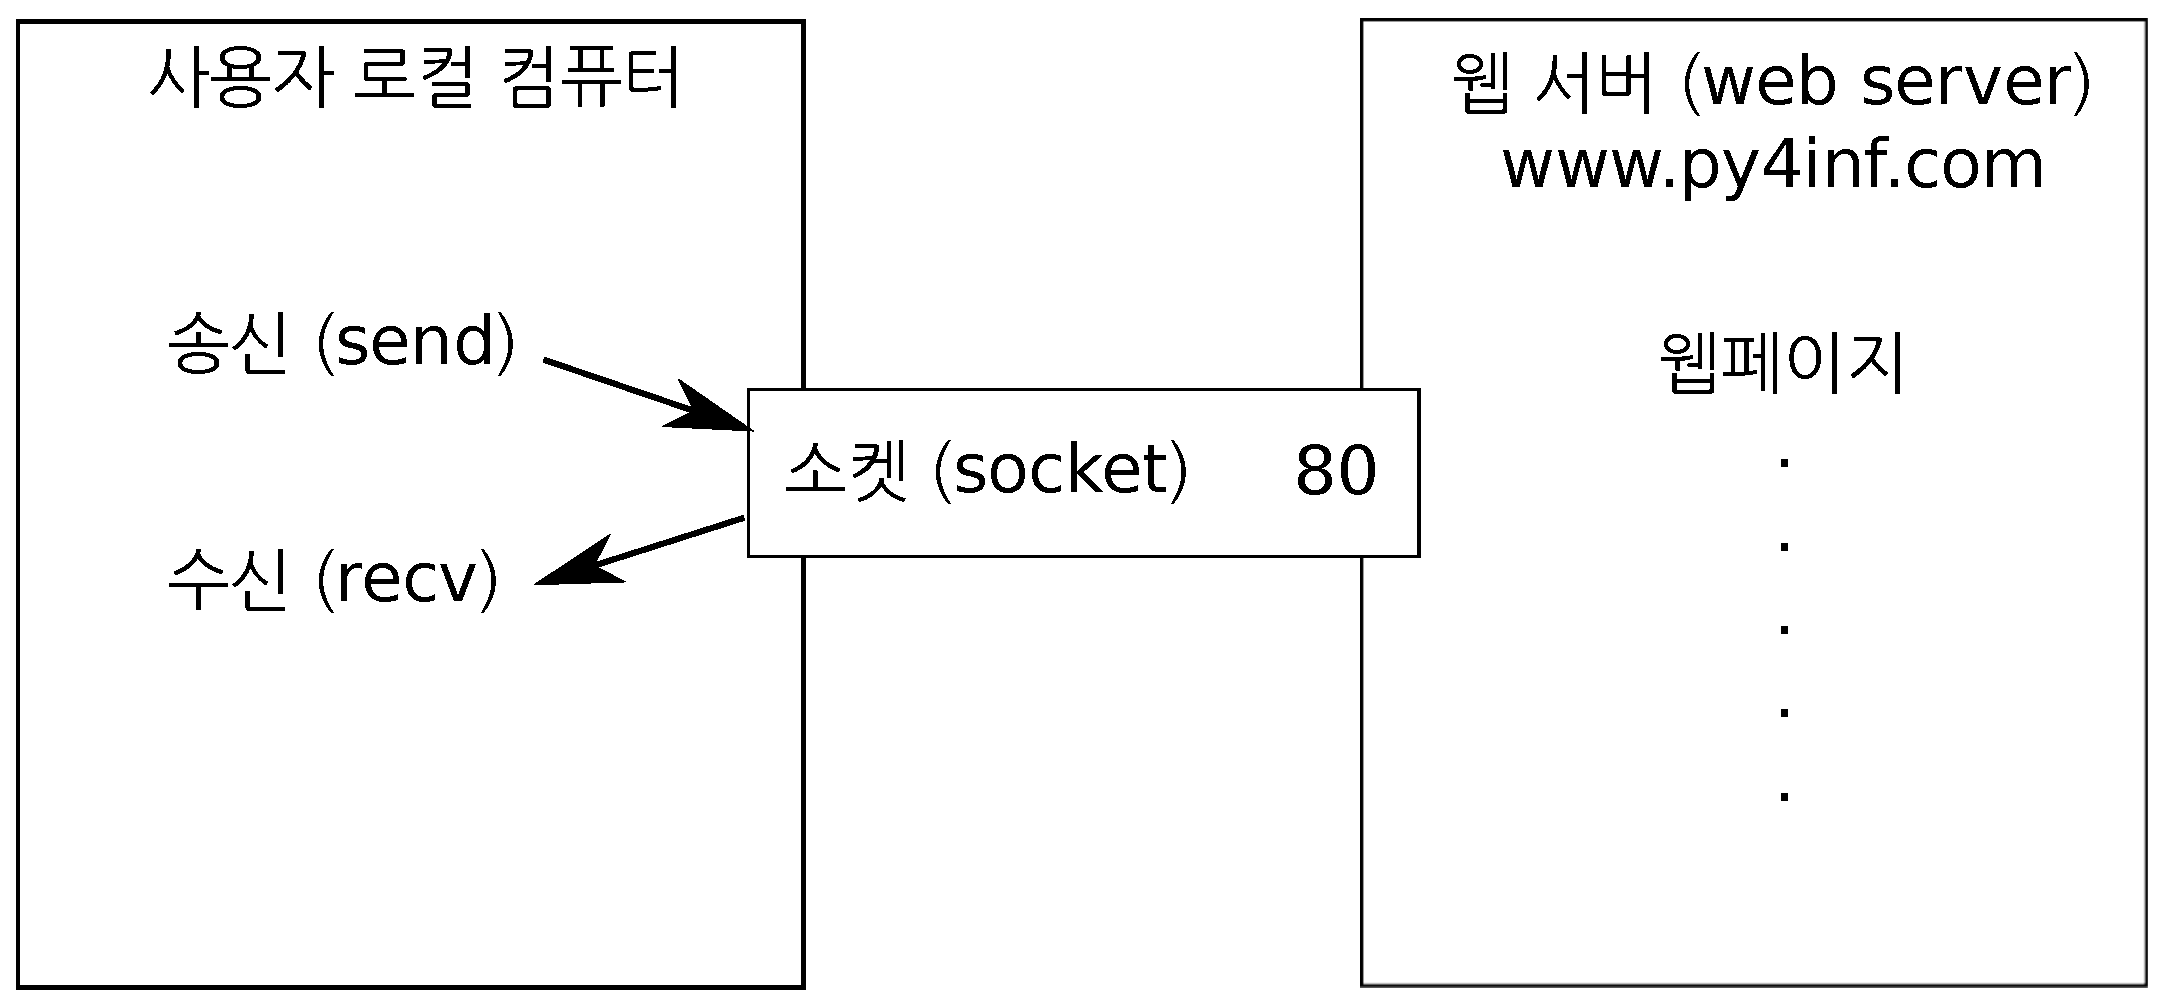
\includegraphics[height=1.50in]{figs2/socket.eps}}
\afterfig

공백 라인을 보내자 마자, 512 문자 덩어리의 데이터를 소켓에서 받아 더 이상 읽을 데이터가 없을 때까지(즉, recv()이 빈 문자열을 반환한다.) 데이터를 출력하는 루프를 작성한다.

프로그램 실행결과 다음을 얻을 수 있다.

\beforeverb
\begin{verbatim}
HTTP/1.1 200 OK
Date: Sun, 14 Mar 2010 23:52:41 GMT
Server: Apache
Last-Modified: Tue, 29 Dec 2009 01:31:22 GMT
ETag: "143c1b33-a7-4b395bea"
Accept-Ranges: bytes
Content-Length: 167
Connection: close
Content-Type: text/plain

But soft what light through yonder window breaks
It is the east and Juliet is the sun
Arise fair sun and kill the envious moon
Who is already sick and pale with grief
\end{verbatim}
\afterverb
%

출력결과는 웹서버가 문서를 기술하기 위해서 보내는 헤더(header)로 시작한다.
예를 들어, {\tt Content-Type } 헤더는 문서가 일반 텍스트 문서({\tt text/plain})임을 표기한다.

서버가 헤더를 보낸 후에, 빈 라인을 추가해서 헤더 끝임을 표기하고 나서 실제 파일{\tt romeo.txt}을 보낸다.

이 예제를 통해서 소켓을 통해서 저수준(low-level) 네트워크 연결을 어떻게 하는지 확인할 수 있다.
소켓을 사용해서 웹서버, 메일 서버 혹은 다른 종류의 서버와 통신할 수 있다.
필요한 것은 프로토콜을 기술하는 문서를 찾고 프로토콜에 따라 데이터를 주고 받는 코드를 작성하는 것이다.

하지만, 가장 흔히 사용하는 프로토콜은 HTTP (즉, 웹) 프로토콜이기 때문에, 
파이썬에는 HTTP 프로토컬을 지원하기 위해 특별히 설계된 라이브러리가 있다.
이것을 통해서 웹상에서 데이터나 문서를 검색을 쉽게 할 수 있다.

\section{HTTP를 통해서 이미지 가져오기}

\index{urllib!image}
\index{image!jpg}
\index{jpg}

상기 예제에서 파일의 새줄(newline)을 가진 일반 텍스트 파일을 가져와서, 프로그램이 동작할 때 화면상에 데이터를 단순히 복사했다.
HTTP를 사용하여 이미지를 가져오는 비슷한 프로그램을 작성할 수 있다. 프로그램 실행 시에 화면에 데이터를 복사하는 대신에,
문자열로 데이터를 쌓고, 다음과 같이 헤더를 잘라내고 나서 파일에 이미지 데이터를 저장한다. 

\beforeverb
\begin{verbatim}
import socket
import time

mysock = socket.socket(socket.AF_INET, socket.SOCK_STREAM)
mysock.connect(('www.py4inf.com', 80))
mysock.send('GET http://www.py4inf.com/cover.jpg HTTP/1.0\n\n')


count = 0
picture = "";
while True:
    data = mysock.recv(5120)
    if ( len(data) < 1 ) : break
    # time.sleep(0.25)
    count = count + len(data)
    print len(data),count
    picture = picture + data

mysock.close()

# Look for the end of the header (2 CRLF)
pos = picture.find("\r\n\r\n");
print 'Header length',pos
print picture[:pos]

# Skip past the header and save the picture data
picture = picture[pos+4:]
fhand = open("stuff.jpg","wb")
fhand.write(picture);
fhand.close()
\end{verbatim}
\afterverb
%

프로그램을 실행하면, 다음과 같은 출력을 생성한다.

\beforeverb
\begin{verbatim}
$ python urljpeg.py 
2920 2920
1460 4380
1460 5840
1460 7300
...
1460 62780
1460 64240
2920 67160
1460 68620
1681 70301
Header length 240
HTTP/1.1 200 OK
Date: Sat, 02 Nov 2013 02:15:07 GMT
Server: Apache
Last-Modified: Sat, 02 Nov 2013 02:01:26 GMT
ETag: "19c141-111a9-4ea280f8354b8"
Accept-Ranges: bytes
Content-Length: 70057
Connection: close
Content-Type: image/jpeg
\end{verbatim}
\afterverb
%
{\tt Content-Type } 헤더가 문선의 본문이 이미지({\tt image/jpeg})를 나타내는 것을 볼 수 있다.
프로그램이 완료되면, 이미지 뷰어로 {\tt stuff.jpg} 파일을 열어서 이미지 데이터를 볼 수 있다.

프로그램을 실행하면, {\tt recv()} 메쏘드를 호출할 때 마다 5120 문자를 얻지 못하는 것을 볼 수 있다.
{\tt recv()} 호출하는 매 순간 웹서버에서 네트워크로 전송되는 가능한 많은 문자를 받게 된다. 
5120 문자까지 요청을 매번 하지만, 1460 혹은 2920 문자를 얻는다. 

결과값은 네트워크 속도에 따라 달라질 수 있다. {\tt recv()} 메쏘드의 마지막 호출에는 스트림 끝에 1681 바이트만 받았고,
{\tt recv()} 다음 호출에는 0 길이 문자열을 얻게 되어서 서버가 소켓의 마지막에 {\tt close()}를 호출하고 
더이상 데이터가 없다는 것을 알려준다.

\index{time}
\index{time.sleep}

주석처리한 {\tt time.sleep()}을 풀어줌으로써 {\tt recv()} 연속 호출을 늦출 수 있다.
이런 방식으로 매 호출 후에 0.25초 기다리게 함으로서 서버가 먼저 도축할 수 있어서 더 많은 데이터를 
사용자가 {\tt recv()} 호출하기 전에 보낼 수가 있다.
지연을 넣어서 프로그램을 다시 실행하면 다음과 같다.

\beforeverb
\begin{verbatim}
$ python urljpeg.py 
1460 1460
5120 6580
5120 11700
...
5120 62900
5120 68020
2281 70301
Header length 240
HTTP/1.1 200 OK
Date: Sat, 02 Nov 2013 02:22:04 GMT
Server: Apache
Last-Modified: Sat, 02 Nov 2013 02:01:26 GMT
ETag: "19c141-111a9-4ea280f8354b8"
Accept-Ranges: bytes
Content-Length: 70057
Connection: close
Content-Type: image/jpeg
\end{verbatim}
\afterverb
%

{\tt recv()} 호출에 처음과 마지막을 제외하고, 매번 새로운 데이터를 요청할 때마다 이제는 5120 문자를 얻는다. 

서버 {\tt send()} 요청과 응용프로그램 {\tt recv()} 요청 사이에 버퍼가 있다.
프로그램에 지연을 넣어 실행하게 될 때, 어느 지점엔가 서버가 소켓의 버퍼를 채우고 응용프로그램이 버퍼를 비울 때까지
잠시 멈춰야 된다. 보내는 응용프로그램 혹은 받는 응용프로그램을 멈추는 행위를 ''흐름 제어(flow control)''이라고 한다.

\index{flow control}

\section{{\tt urllib} 사용하여 웹페이지 가져오기}

수작업으로 소켓 라이브러리를 사용하여 HTTP로 데이터를 보내거나 받을 수 있지만,
{\tt urllib} 라이브러리를 사용하여 파이썬에서 동일한 작업을 수행하는 좀더 간편한 방식이 있다.

{\tt urllib}을 사용하여 파일처럼 웹페이지를 다룰 수가 있다.
단순하게 어느 웹페이지를 가져오늘 것인지만 지정하면 {\tt urllib} 라이브러리가 모든 HTTP 프로토콜과 헤더관련 사항을 처리해 준다.

{\tt urllib}를 사용하여 웹으로부터 {\tt romeo.txt} 파일을 읽는 상응하는 코드는 다음과 같다.

\beforeverb
\begin{verbatim}
import urllib

fhand = urllib.urlopen('http://www.py4inf.com/code/romeo.txt')
for line in fhand:
   print line.strip()
\end{verbatim}
\afterverb
%

{\tt urllib.urlopen}으로 웹페이지를 열게 되면, 파일처럼 다룰 수 있고 {\tt for} 루프를 사용하여 데이터를 읽을 수 있다.

프로그램을 실행하면, 파일 내용의 출력만을 볼 수 있다. 헤더정보가 여전히 보내지지만, {\tt urllib} 코드가 헤더를 받아 내부적으로 처리하고,
단지 데이터만 사용자에게 반환한다.

\beforeverb
\begin{verbatim}
But soft what light through yonder window breaks
It is the east and Juliet is the sun
Arise fair sun and kill the envious moon
Who is already sick and pale with grief
\end{verbatim}
\afterverb
%

예제로, {\tt romeo.txt} 데이터를 가져와서 파일의 각 단어의 빈도를 계산하는 프로그램을 다음과 같이 작성할 수 있다.

\beforeverb
\begin{verbatim}
import urllib

counts = dict()
fhand = urllib.urlopen('http://www.py4inf.com/code/romeo.txt')
for line in fhand:
    words = line.split()
    for word in words:
        counts[word] = counts.get(word,0) + 1   
print counts
\end{verbatim}
\afterverb
%

다시 한번, 웹페이지를 열게 되면, 로컬 파일처럼 웹페이지를 읽을 수 있다.

\section{HTML 파싱과 웹 스크래핑}

\index{web!scraping}
\index{parsing HTML}

파이썬 {\tt urllib} 활용하는 흔한 사례는 웹 {\bf 스크래핑(scraping)}이다.
웹 스크래핑은 웹브라우저를 가장하여 웹페이지를 가져와서 페이지 내부의 데이터를 살펴보고 패턴을 찾은 프로그램을 작성하는 것이다.
예로, 구글같은 검색엔진은 웹 페이지의 소스를 찾아서 다른 페이지로의 링크를 추출하고, 다른 페이지를 가져와서 링크를 추출하는 일을 반복한다.
이러한 기법으로 구글은 웹상의 거의 모든 페이지를 {\bf 거미(spiders)}줄처럼 연결한다.

구글은 또한 다른 페이지로 연결되는 링크의 빈도를 사용하여 얼마나 중요한 페이지인지를 측정하고 
페이지가 검색결과에 얼마나 높이 나타낸다.

\section{정규 표현식 사용 HTML 파싱하기}

HTML을 파싱하는 한가지 간단한 방식은 정규 표현식을 사용하여 특정한 패턴과 매칭하는 부속문자열을 반복적으로 찾아 추출하는 것이다.

여기 간단한 웹페이지가 있다.

\beforeverb
\begin{verbatim}
<h1>The First Page</h1>
<p>
If you like, you can switch to the
<a href="http://www.dr-chuck.com/page2.htm">
Second Page</a>.
</p>
\end{verbatim}
\afterverb
%

상기 웹페이지에서 링크를 찾아 추출하는 적격의 정규표현식을 다음과 같이 구성할 수 있다.

\beforeverb
\begin{verbatim}
href="http://.+?"
\end{verbatim}
\afterverb
%

작성된 정규 표현식은 ``href="http://''로 시작하고, 하나 혹은 이상의 ``.+?'' 문자를 가지고 큰 따옴표를 가진 문자열을 찾는다.
``.+?''에 물음표는 매칭이 ''욕심(greedy)'' 방식보다 ''비욕심(non-greedy)'' 방식으로 수행됨을 나타낸다. 
비욕심 매칭방식은 가능한 가장 작게 매칭되는 문자열을 찾는 방식이고, 욕심 방식은 가능한 가장 크게 매칭되는 문자열을 찾는 방식이다.

\index{greedy}
\index{non-greedy}

추출하고자 하는 문자열의 어느부분인지를 표기하기 위해서 정규 표현식에 괄호를 추가하여 다음과 같이 프로그램을 작성한다.

\index{regex!parentheses}
\index{parentheses!regular expression}

\beforeverb
\begin{verbatim}
import urllib
import re

url = raw_input('Enter - ')
html = urllib.urlopen(url).read()
links = re.findall('href="(http://.*?)"', html)
for link in links:
    print link
\end{verbatim}
\afterverb
%

{\tt findall} 정규 표현식 메쏘드는 정규 표현식과 매칭되는 모든 문자열 리스트를 추출하여 큰 따옴표 사이에 링크 텍스트만을 반한한다.

프로그램을 실행하면, 다음 출력을 얻게된다.

\beforeverb
\begin{verbatim}
python urlregex.py 
Enter - http://www.dr-chuck.com/page1.htm
http://www.dr-chuck.com/page2.htm

python urlregex.py 
Enter - http://www.py4inf.com/book.htm
http://www.greenteapress.com/thinkpython/thinkpython.html
http://allendowney.com/
http://www.py4inf.com/code
http://www.lib.umich.edu/espresso-book-machine
http://www.py4inf.com/py4inf-slides.zip
\end{verbatim}
\afterverb
%

정규 표현식은 HTML이 예측가능하고 잘 구성된 경우에 멋지게 작동한다.
하지만, ''망가진'' HTML 페이지가 많아서, 정규 표현식만을 사용하는 솔류션은 유효한 링크를 놓치거나 잘못된 데이터를 찾게 되는 것으로 끝날 수 있다.

이 문제는 강건한 HTML 파싱 라이브러리를 사용해서 해결될 수 있다.

\section{BeautifulSoup 사용한 HTML 파싱}
\index{BeautifulSoup}

HTML을 파싱하여 페이지에서 데이터를 추출할 수 있는 파이썬 라이브러리는 많이 있다.
각각의 라이브러리는 강점과 약점이 있어서 사용자 필요에 따라 취사선택하여야 한다.

예로, 간단하게 HTML 입력을 파싱하여 {\bf BeautifulSoup} 라이브러리를 사용하여 링크를 추출할 것이다.
다음 웹사이트에서 BeautifulSoup 코드를 다운로드 받아 설치할 수 있다.

\url{www.crummy.com}

BeautifulSoup 라이브러리를 다운로드 받아 ''설치''하거나 {\tt BeautifulSoup.py} 파일을 응용프로그램과 동일한 폴더에 놓을 수 있다.

HTML이 XMX 처럼 보이고 몇몇 페이지는 XML로 되도록 꼼꼼하게 구축되었지만, 대부분의 HTML은 통상 잘못 구축되어서 XML 파서가 HTML 전체 페이지를 
잘못 구성된 것으로 거부한다. BeautifulSoup 라이브러리는 결점 많은 HTML 페이지에 내성이 있어서 사용자가 필요로하는 데이터를 쉽게 추출할 수 있게 한다.

{\tt urllib}를 사용하여 페이지를 읽어들이고, {\tt BeautifulSoup}를 사용하여 앵커 태그 ({\tt a})로 {\tt href} 속성을  추출합니다.

\index{BeautifulSoup}
\index{HTML}
\index{parsing!HTML}

\beforeverb
\begin{verbatim}
import urllib
from BeautifulSoup import *

url = raw_input('Enter - ')
html = urllib.urlopen(url).read()
soup = BeautifulSoup(html)

# Retrieve all of the anchor tags
tags = soup('a')
for tag in tags:
   print tag.get('href', None)
\end{verbatim}
\afterverb
%

프로그램이 웹 주소를 입력받고, 웹페이지를 열고, 데이터를 읽어서 BeautifulSoup 파서에 전달하고,
그리고 나서 모든 앵커 태그를 불러와서 각 태그에 {\tt href} 속성을 출력한다.

프로그램을 실행하면, 아래와 같다.

\beforeverb
\begin{verbatim}
python urllinks.py 
Enter - http://www.dr-chuck.com/page1.htm
http://www.dr-chuck.com/page2.htm

python urllinks.py 
Enter - http://www.py4inf.com/book.htm
http://www.greenteapress.com/thinkpython/thinkpython.html
http://allendowney.com/
http://www.si502.com/
http://www.lib.umich.edu/espresso-book-machine
http://www.py4inf.com/code
http://www.pythonlearn.com/
\end{verbatim}
\afterverb
%

BeautifulSoup을 사용하여 다음과 같이 각 태그의 다양한 부분을 뽑아낼 수 있다.

\beforeverb
\begin{verbatim}
import urllib
from BeautifulSoup import *

url = raw_input('Enter - ')
html = urllib.urlopen(url).read()
soup = BeautifulSoup(html)

# Retrieve all of the anchor tags
tags = soup('a')
for tag in tags:
   # Look at the parts of a tag
   print 'TAG:',tag
   print 'URL:',tag.get('href', None)
   print 'Content:',tag.contents[0]
   print 'Attrs:',tag.attrs
\end{verbatim}
\afterverb
%

상기 프로그램은 다음을 출력합니다.

\beforeverb
\begin{verbatim}
python urllink2.py 
Enter - http://www.dr-chuck.com/page1.htm
TAG: <a href="http://www.dr-chuck.com/page2.htm">
Second Page</a>
URL: http://www.dr-chuck.com/page2.htm
Content: [u'\nSecond Page']
Attrs: [(u'href', u'http://www.dr-chuck.com/page2.htm')]
\end{verbatim}
\afterverb
%

HTML을 파상하는데 BeautifulSoup이 가진 강력한 기능을 예제로 보여줬습니다.
좀더 자세한 사항은 \url{www.crummy.com} 에서 문서와 예제를 살펴보세요.

\section{urllib을 사용하여 바이너리 파일 읽기}

이미지나 비디오 같은 텍스트가 아닌 (혹은 바이너리)파일을 가져올 때가 종종 있다.
이런 파일의 데이터는 일반적으로 출력하는 것은 유용하지 않다. 하지만, {\tt urllib}을 사용하여,
하드 디스크의 로컬 파일에 URL 사본을 쉽게 만들 수 있다.

\index{binary file}

패턴은 URL을 열고, {\tt read}를 사용해서 문서 전체의 내용을 다운로드하여 문자열 변수({\tt img})에 다운로드하고,
그 정보를 다음과 같이 로컬 파일에 쓴다.

\beforeverb
\begin{verbatim}
img = urllib.urlopen('http://www.py4inf.com/cover.jpg').read()
fhand = open('cover.jpg', 'w')
fhand.write(img)
fhand.close()
\end{verbatim}
\afterverb
%

작성한 프로그램은 네트워크로 모든 데이터를 한번에 읽어서 컴퓨터 주기억장치의 {\tt img} 변수에 저장하고,
{\tt cover.jpg} 파일을 열어 디스크에 데이터를 쓴다. 이 방식은 파일의 크기가 사용자 컴퓨터의 메모리 크기보다 작으면 정상적으로 작동한다.

하지만, 큰 오디오 혹은 비디오 파일이라면, 상기 프로그램은 멈추거나 사용자 컴퓨터가 메모리가 부족할 때 극단적으로 느려질 수 있다.
메모리 부족을 피하기 위해서, 데이터를 블럭 혹은 버퍼로 가져오고 다음 블럭을 가져오기 전에 디스크에 각각의 브럭을 쓴다.
이런 방식으로 사용자가 가진 모든 메모리를 사용하지 않고 임의 크기의 파일을 읽어올 수 있다.

\beforeverb
\begin{verbatim}
import urllib

img = urllib.urlopen('http://www.py4inf.com/cover.jpg')
fhand = open('cover.jpg', 'w')
size = 0
while True:
    info = img.read(100000)
    if len(info) < 1 : break
    size = size + len(info)
    fhand.write(info)

print size,'characters copied.'
fhand.close()
\end{verbatim}
\afterverb
%

상기 예제에서, 한번에 100,000 문자만 읽어 오고, 웹에서 다음 100,000 문자를 가져오기 전에 {\tt cover.jpg} 파일에 읽어온 문자를 쓴다.

프로그램 실행 결과는 다음과 같다.

\beforeverb
\begin{verbatim}
python curl2.py 
568248 characters copied.
\end{verbatim}
\afterverb
%

UNIX 혹은 매킨토시 컴퓨터를 가지고 있다면, 다음과 같이 이러한 동작을 수행하는 명령어가 운영체제에 내장되어 있다.

\index{curl}

\beforeverb
\begin{verbatim}
curl -O http://www.py4inf.com/cover.jpg
\end{verbatim}
\afterverb
%

{\tt curl}은 ``copy URL''의 단축 명령어로 두 예제는 {\tt curl} 명령어와 비슷한 기능을 구현해서, 
\url{www.py4inf.com/code} 사이트에 {\tt curl1.py}, {\tt curl2.py} 이름으로 올라가 있다.
동일한 작업을 좀더 효과적으로 수행하는 {\tt curl3.py} 샘플 프로그램도 있어서 실질적으로 작성하는 프로그램에 이런한 패턴을 이용하여 구현할 수 잇다.

\section{용어정의}

\begin{description}

\item[BeautifulSoup:] 파이썬 라이브러리로 HTML 문서를 파싱하고 
브라우저가 일반적으로 생략하는 HTML의 불완전한 부분을 보정하여 HTML 문서에서 데이터를 추출한다.
\url{www.crummy.com} 사이트에서 BeautifulSoup 코드를 다운로드 받을 수 있다.

\index{BeautifulSoup}

\item[포트(port):] 서버에 소켓 연결을 할 때, 사용자가 어느 응용프로그램을 연결하는지 나타내는 숫자.
예로, 웹 트래픽은 통상 80 포트, 전자우편은 25 포트를 사용한다.

\index{port}

\item[스크랩(scrape):] 프로그램이 웹브라우저를 가장하여 웹페이지를 가져오고 웹 페이지의 내용을 검색한다.
종종 프로그램이 한 페이지의 링크를 따라 다른 페이지를 찾아서 웹페이지 네트워크 혹은 소셜 네트워크 전체를 훑을 수 있다.

\index{socket}

\item[소켓(socket):] 두 응용프로그램 사이의 네트워크 연결. 두 응용프로그램은 양 방향으로 데이터를 주고 받는다.
\index{socket}

\item[스파이더(spider):] 검색 색인을 구축하기 위해서 한 웹페이지에서 그 페이지에 링크된 모든 페이지를 가져오기를 반복하여
거의 모든 인터넷의 모든 페이지를 가져오기 위해서 사용하는 검색엔진 행동.
\index{spider}

\end{description}

\section{연습문제}

\begin{ex}
소켓 프로그램 {\tt socket1.py}을 변경하여 임의의 웹페이지를 읽을 수 있도록 URL을 사용자가 입력하도록 바꾸세요.
{\tt split('/')}을 사용하여 URL을 컴포턴트로 쪼개서 소켓 {\tt connect} 호출에 대해 호스트 명을 추출할 수 있다.
사용자가 적절하지 못한 형식 혹은 존재하지 않는 URL을 입력하는 경우를 다룰 수 있도록 {\tt try}, {\tt except}를 사용하여 오류 검사기능을 추가하세요.
\end{ex}

\begin{ex}
소켓 프로그램을 변경하여 받은 문자갯수를 세고 3000 문자를 출력한 후에 더이상의 텍스트를 출력을 멈추게 하세요.
프로그램은 전체 문서를 가져와야 하고 전체 문자 갯수를 세고, 문서 마지막에 문자 갯수를 출력해야 합니다.
\end{ex}

\begin{ex}
{\tt urllib}을 사용하여 앞의 예제를 반복하세요. (1) 사용자가 입력한 URL에서 문서 가져오기
(2) 3000 문자까지 화면에 보여주기 (3) 문서의 전체 문자 갯수 세기.
이 예제에서 헤더에 대해서는 걱정하지 말고, 단지 문서 본문에서 첫 3000 문자만 화면에 출력하세요.
\end{ex}

\begin{ex} {\tt urllinks.py} 프로그램을 변경하여 가져온 HTML 문서에서 문단 (p) 태그를 추출하고
프로그램의 출력물로 문단 숫자를 세고 화면에 출력하세요. 문단 텍스트를 화면에 출력하지 말고 단지 숫자만 셉니다.
작성한 프로그램을 작은 웹페이지 뿐만 아니라 조금 큰 웹 페이지에도 테스트해 보세요.
\end{ex}

\begin{ex}
(고급) 소켓 프로그램을 변경하여 헤더와 빈 라인을 받은 후에 데이터만 보여지게 하세요.
{\tt recv}는 라인이 아니라 문자(새줄(newline)과 모든 문자)를 받는다는 것을 기억하세요.
\end{ex}


